\section{Dimensionierungen}

\subsection{Widerstände}

\begin{frame}
	\frametitle{Ausgangsseite ($R_C, R_E$) bestimmen}
		\begin{block}{Richtwert für $R_C$}
			Der Richtwert gibt an, dass
			\[R_C < 0.3 \cdot R_L \]
			gelten muss.
		\end{block}
			$\Rightarrow R_C = 0.3 \cdot 22k \Omega = 6.6k \Omega$
			$\xrightarrow{E12} 5.6k \Omega$

		\[ R_E = \frac{\beta \cdot R_C - V_U \cdot R_{BE}}
		{V_U \cdot (1+\beta)} \approx \frac{R_C}{V_U} =
		\frac{5.6k \Omega}{5.62} = 
		996.4 \Omega \xrightarrow{E12} 1k \Omega \]
\end{frame}

\begin{frame}
	\frametitle{Ausgangsseite prüfen}
		\begin{block}{Regel für $\frac{R_C}{R_E}$}
			Die Regel besagt, dass 
			\[ \frac{R_C}{R_E} < 10 \]
			sein muss. Ist dies nicht gegeben, so muss zum
			Emitterwiderstand ein RC-Glied parallel geschaltet
			werden.	
		\end{block}
		\[ \frac{R_C}{R_E} = \frac{5.6k \Omega}{1k \Omega} = 5.6 \]
		$\Rightarrow$ Wir brauchen kein zusätzliches RC-Glied.
				
\end{frame}

\begin{frame}
	\frametitle{Arbeitspunkt bestimmen}
		Wir nehmen als Arbeitspunkt $\frac{U_B}{2}$ an da die
		Sättigungsspannung klein ist für kleine Ströme.
		\begin{figure}
			\centering
				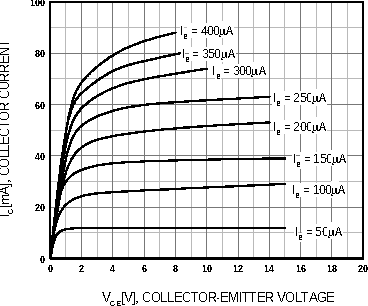
\includegraphics{BC550_Ic_Uce.pdf}
			\caption{$I_C$ vs. $U_{CE}$, BC550}
		\end{figure}
\end{frame}

\begin{frame}
	\frametitle{Bestimmung der Spannung $U_{R_E}$}
	\[ U_{BGND} = U_{BE} + U_{R_E}, \quad
		\text{aus Datenblatt } U_{BE} \approx 660mV \]
	\[ U_{R_E} = R_E \cdot (I_C + I_B), \quad 
		I_C = \frac{\frac{1}{2} \cdot U_B}{R_C} \approx 1.8mA \]
	\[ U_{R_E} = 1k \Omega \cdot (1.8mA + I_B) \xrightarrow{I_B \approx 0}
		U_{R_E} \approx 1k \Omega \cdot 1.8mA = 1.78V\]
	\[ U_{BGND} = 660mV + 1.78V = 2.45V \]
\end{frame}
	
\begin{frame}
	\frametitle{Dimensionierung von $R_1, R_2$}
	\begin{block}{Regel für $I_B$}
		Die Regel besagt, dass
		\[ \frac{I_q}{I_B} = n, \quad 3<n<10 \]
%		sein sollte.
	\end{block}
	\[ \text{Annahme } n = 6 \Rightarrow I_q = n \cdot I_B =
		6 \cdot 8.93 \mu A = 53.57 \mu A \]
	\[ \Rightarrow R_2 = \frac{U_{BGND}}{I_{R_2}} = 
		\frac{2.45V}{53.57 \mu A} = 45.65k \Omega 
		\xrightarrow{E12} 47k \Omega \]
	\[ \Rightarrow R_1 = \frac{U_{R_1}}{I_{R_1}} = 
		\frac{U_B - U_{BGND}}{I_q + I_B} =
		\frac{20V - 2.45V}{8.93 \mu A + 53.57 \mu A} = 
		280.9k \Omega \] 
	\[ R_1 \xrightarrow{E12} 270k \Omega\]
\end{frame}

\subsection{Eingangswiderstand}
\begin{frame}
	\frametitle{Eingangswiderstand}
		Für die Berechnung des Eingangswiderstandes kann $X_C = 0$
		angenommen werden.

		\begin{figure}
			\centering
			\begin{circuitikz}[scale=0.75, transform shape]\draw
				(0,2)	node[anchor=east]{$U_q$}
				(0,2)	to[short, o-]
				(0,2)	to[R=$R_q$, -*]	(2,2)
				(2,2)	to[R=$R_1$]	(2,0)
				(2,2)	to[short, -*]	(4,2)
				(4,2)	to[R=$R_2$]	(4,0)
				(4,2)	to[R=$r_{BE}$]	(6,2)
				(6,2)	to[R=$R_E$]	(6,0)
				(2,0)	node[rground]{}
				(4,0)	node[rground]{}
				(6,0)	node[rground]{}
				;
			\end{circuitikz}
			\caption{Ersatzschaltbild des Verstärkreingangs}
		\end{figure}

\end{frame}

\begin{frame}
	\frametitle{Transformation des Eingangswiderstandes}
		\[ R_e = \frac{1}{\frac{1}{R_1} + 
			\frac{1}{R_2} + 
			\frac{1}{r_{BE} + R_E}} \] 
		\[ r_e^t = r_{BE} + (\beta + 1) \cdot R_e, \quad 
			r_{BE} \xrightarrow{Datenblatt} 8.7k \Omega \]
		\[ r_e = \frac{1}{\frac{1}{r_e^t} + 
			\frac{1}{R_1} +
			\frac{1}{R_2}}
			= 37.57k \Omega\]
\end{frame}

\subsection{DC-Entkopplung}
\begin{frame}
	\frametitle{Berechnung der DC-Entkopplung}
	\[ f_{g_{UE}} = \frac{1}{2 \cdot \pi \cdot (r_e + R_q) \cdot C_q} \]
	\[ \Rightarrow C_q = 423nF \xrightarrow{E12} 470nF \]
	\[ f_{g_{UA}} = \frac{1}{2 \cdot \pi \cdot (r_a + R_L) \cot C_A} \]
	\[ \Rightarrow C_A = 577nF \xrightarrow{E12} 680nF \]
\end{frame}

\subsection{Verstärkung}
\begin{frame}
	\frametitle{Verstärkung}
	\[ \frac{U_a}{U_q} = \frac{R_a}{R_e} = 
		\frac{-3 \cdot \frac{R_C \cdot R_L}{R_C + R_L}}{R_q + R_e} 
		= -0.46 \]
\end{frame}

